
\section{拟凝聚层的拉回：三种视角}

我们接下来讨论\trQCSheaf{}的拉回：若 $\pi\colon X\to Y$ 是\trScheme{}之间的一个\trMorphism，则 $\pi^*$ 是一个\trCovariantFunctor{} $\mathit{QCoh}_Y\to\mathit{QCoh}_X$。（事实上，我们的讨论可直接照搬适用于\trRingedSpace{}上 $\OO$-\trModule{}的拉回；见 \S14.5.5 与 \S14.5.6。）\trQCSheaf{}的拉回这个概念，第一眼（第二眼也一样）容易让人迷惑。（比如，它\emph{并非}\trInverseImage\trSheaf，尽管我们会看到它与之有关。）

\textbf{14.5.1.}\quad 下面是三个你已在其中见过拉回、或者能够很快理解拉回的语境。把它们记在心里或许会有帮助，好让你在接下来这场漫长的讨论中有所锚定。设 $\mathscr{G}$ 是\trScheme{} $Y$ 上的一个\trQCSheaf。
\begin{enumerate}[label=(\roman*)]
\item \emph{（到\trOpenSubset{}上的限制）}若 $i\colon\mathrm{U}\hookrightarrow Y$ 是一个\trOpenEmbedding，则 $i^*\mathscr{G}$ 就是 $\mathscr{G}\vert_{\mathrm{U}}$，即 $\mathscr{G}$ 到 $\mathrm{U}$ 上的\trRestriction（\mbox{例~2.2.8}）。
\item \emph{（到点上的限制）}若 $i\colon p\hookrightarrow Y$ 是点 $p$ 在 $Y$ 中的「\trInclusionMap」（比如说，一个\trClosedPoint{}的\trClosedEmbedding；见\cref{ex:spec-local-ring-canonical-map}(b)），则 $i^*\mathscr{G}$ 就是 $\mathscr{G}\vert_p$，即 $\mathscr{G}$ 在 $p$ 处的\trFiber（定义~4.3.8）。
\end{enumerate}
记号 $\mathscr{G}\vert_{\mathrm{U}}$ 与 $\mathscr{G}\vert_p$ 的相似，恰恰是因为二者都是拉回。拉回（尤其是到\trLocally\trClosedSubscheme{}或\trGenericPoint{}上的拉回）常被称为\emph{\trRestriction}。正因如此，若 $\pi\colon X\to Y$ 是某种\trInclusionMap{}（比如一个\trLocallyClosedEmbedding，或者「\trGenericPoint{}的\trInclusionMap」），则当 $\pi$ 可被解读为某种「包含」时，$\pi^*\mathscr{G}$ 常被写作 $\mathscr{G}\vert_X$，并称为\textbf{$\mathscr{G}$ 到 $X$ 上的\trRestriction}。
\begin{enumerate}[label=(\roman*)]\setcounter{enumi}{2}
\item \emph{（拉回\trVectorBundle）}设 $\mathscr{G}$ 是 $Y$ 上的一个\trLocallyFreeSheaf，而 $\pi\colon X\to Y$ 是任意\trMorphism。那么 $\pi^*\mathscr{G}$ 就是 $\mathscr{G}$ 作为\trVectorBundle{}的拉回，如 \S14.1.7 中所定义。（这将在 \S14.5.6 中得到建立。）
\end{enumerate}

\textbf{14.5.2.}\ \emph{策略。}\quad 我们将会看到关于拉回的三种不同思考方式。每一种都有显著的缺点，但合在一起便能给出一个良好的理解。
\begin{enumerate}[label=(\alph*)]
\item 由于我们是通过\trAffine\trOpenSet{}与相应\trRing{}上的\trModule{}来理解\trQCSheaf{}的，我们便先给出这一路线下的一个解读。这对于证明与理解各种事实将非常有用。缺点则是：想据此做出一个定义（当靶不是\trAffine{}的时候）会很烦人，因为粘合论证可能相当繁琐。
\item 正如我们在\trFiberProduct{}中所见，借助\trUniversalProperty{}可以让粘合论证变得简单些，所以我们的第二个「定义」将由\trUniversalProperty{}给出。这很优雅，但缺点在于：它仍然需要一个构造，而且由于它是在更大的 $\OO$-\trModule{}范畴中运作的，从\trUniversalProperty{}本身看不出来它把\trQCSheaf{}送到\trQCSheaf。不过若靶是\trAffine{}的，则容易看出我们 (a) 中的构造满足该\trUniversalProperty。

再者，这个泛性质「对靶是局部的」：若 $\pi\colon X\to Y$ 是任意\trMorphism，$i\colon\mathrm{U}\hookrightarrow Y$ 是一个\trOpenEmbedding，而 $\mathscr{G}$ 是 $Y$ 上的一个\trQCSheaf，那么只要 $\pi^*\mathscr{G}$ 存在，它在 $\pi^{-1}(\mathrm{U})$ 上的\trRestriction{}便（典范地等同于）$(\pi|_{\mathrm{U}})^*(\mathscr{G}|_{\mathrm{U}})$。于是，倘若拉回在一般情形下存在（哪怕只是作为 $\OO$-\trModule），那么在 $Y$ 上仿射局部地看，它就像 (a) 中的那个构造（从而是\trQC{}的）。
\item 第三个定义则是对一般\trRingedSpace{}都行之有效的一种。它很简短，而且容易看出它满足该\trUniversalProperty。它并不显然把\trQCSheaf{}送到\trQCSheaf（至少按我们定义\trQCSheaf{}的那种方式来看是如此）——先验地，它把\trQCSheaf{}送到 $\OO$-\trModule。但多亏上文 (b) 末尾借助 (a) 的那番讨论，这便表明\trQCSheaf{}的拉回确实是\trQC{}的。
\end{enumerate}

\textbf{14.5.3.\ 用仿射描述拉回的首次尝试。}\quad 设 $\pi\colon X\to Y$ 是\trScheme{}之间的一个\trMorphism，而 $\mathscr{G}$ 是 $Y$ 上的一个\trQCSheaf。我们想用 $X$ 与 $Y$ 上的\trAffine\trOpenSet{}来定义拉回\trQCSheaf{} $\pi^*\mathscr{G}$。设 $\Spec A\subset X$ 与 $\Spec B\subset Y$ 是\trAffine\trOpenSet，满足 $\pi(\Spec A)\subset\Spec B$。设 $\mathscr{G}\vert_{\Spec B}\cong\widetilde{N}$。拉回应当与\trTensorProduct{}发生关系——或许正是这一点给了我们动机——我们想要
\begin{equation*}\tag{14.5.3.1}\label{eq:pullback-sections-tensor}
\Gamma(\Spec A,\pi^*\mathscr{G})=N\otimes_B A.
\end{equation*}
更精确地说，我们想把 $\Gamma(\Spec A,\pi^*\mathscr{G})$ 与 $N\otimes_B A$ 等同起来。这可以意味着：我们用它来构造 $\pi^*\mathscr{G}$ 的一个定义，办法是「把所有这些信息粘合在一起」（并证明它是\trWellDefined{}的）。也可以意味着：我们以某种别的方式定义 $\pi^*\mathscr{G}$，然后再找出一个\trNatural{}的等同 \eqref{eq:pullback-sections-tensor}。第一条路线可以走得通（\S14.5.4 便是第一步），但我们将沿着第二条路线走。

\begin{figure}[htbp]
\centering
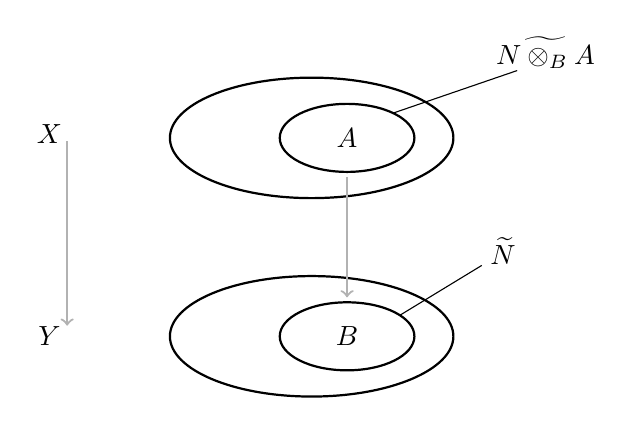
\begin{tikzpicture}[scale=0.9]
  \node at (-1.2,0.1) {$X$};
  \draw[thick] (2.5,0.05) ellipse (2.0 and 0.85);
  \draw[thick] (3.0,0.05) ellipse (0.95 and 0.48);
  \node at (3.0,0.05) {$\Spec A$};
  \node at (-1.2,-2.75) {$Y$};
  \draw[thick] (2.5,-2.75) ellipse (2.0 and 0.85);
  \draw[thick] (3.0,-2.75) ellipse (0.95 and 0.48);
  \node at (3.0,-2.75) {$\Spec B$};
  \draw[gray!60,thick,->] (-0.95,0.0) -- (-0.95,-2.6);
  \draw[gray!60,thick,->] (3.0,-0.5) -- (3.0,-2.2);
  \node at (5.8,1.25) {$\widetilde{N\otimes_B A}$};
  \draw[thin] (5.4,1.0) -- (3.65,0.4);
  \node at (5.2,-1.55) {$\widetilde{N}$};
  \draw[thin] (4.9,-1.75) -- (3.75,-2.45);
\end{tikzpicture}
\caption{拟凝聚层的拉回（模论式）。（依原书手绘图重绘。）}\label{fig:pullback-module-theoretic}
\end{figure}

\textbf{14.5.4.}\quad 我们以\emph{固定}一个\trAffine\trOpenSubset{} $\Spec B\subset Y$ 来启动这项工程。为免混淆，令 $\phi=\pi\vert_{\pi^{-1}(\Spec B)}\colon\pi^{-1}(\Spec B)\to\Spec B$。我们将在 $\pi^{-1}(\Spec B)$ 上定义一个\trQCSheaf，它将被证明就是 $\phi^*(\mathscr{G}\vert_{\Spec B})$（并且也将是 $\pi^*\mathscr{G}$ 限制到 $\pi^{-1}(\Spec B)$ 上的结果）。

若 $\Spec A_f\subset\Spec A$ 是一个\trDistinguishedOpen，则
\[
\Gamma(\Spec A_f,\phi^*\mathscr{G})=N\otimes_B A_f=(N\otimes_B A)_f=\Gamma(\Spec A,\phi^*\mathscr{G})_f,
\]
其中「$=$」意为「典范同构」。定义\trRestrictionMap{} $\Gamma(\Spec A,\phi^*\mathscr{G})\to\Gamma(\Spec A_f,\phi^*\mathscr{G})$，
\begin{equation*}\tag{14.5.4.1}\label{eq:restriction-map-affine-local}
\Gamma(\Spec A,\phi^*\mathscr{G})\longrightarrow\Gamma(\Spec A,\phi^*\mathscr{G})\otimes_A A_f,
\end{equation*}
其为 $\alpha\mapsto\alpha\otimes 1$（当然了）。于是，$\phi^*\mathscr{G}$ 是（或者说：可延拓成）$\pi^{-1}(\Spec B)$ 上的一个\trQCSheaf（据\mbox{练习~6.2.D}）。

现在，对每一个\trAffine\trOpenSubset{} $\Spec B\subset Y$，我们都在 $\pi^{-1}(\Spec B)$ 上定义了一个\trQCSheaf。我们想证明：随着 $\Spec B$ 的变动，这一构造粘合成 $X$ 上单独的一个\trQCSheaf。

欢迎你亲自把这个粘合妥善完成，比如说利用 $Y$ 的\trDistinguishedAffineBase（\S6.2.1）。那样做是可行的，但可能令人迷惑，所以我们另取一条路径。

\textbf{14.5.5.\ 拉回的\trUniversalProperty{}定义。}\quad 设 $\pi\colon X\to Y$ 是\trRingedSpace{}之间的一个\trMorphism，而 $\mathscr{G}$ 是一个 $\OO_Y$-\trModule。（我们当然感兴趣的是 $\pi$ 为\trScheme{}之间的\trMorphism{}而 $\mathscr{G}$ \trQC{}的情形。即便把我们的讨论专门化到\trScheme，其中的大部分也将不加改变地适用于这个更一般的情形。）我们借助如下这条\trAdjointness\trUniversalProperty{}来「定义」拉回 $\pi^*\mathscr{G}$（视作 $\OO_X$-\trModule）：对任意 $\OO_X$-\trModule{} $\mathscr{F}$，存在双射 $\Hom_{\OO_X}(\pi^*\mathscr{G},\mathscr{F})\overset{\sim}{\longleftrightarrow}\Hom_{\OO_Y}(\mathscr{G},\pi_*\mathscr{F})$，并且这些双射对 $\mathscr{F}$ 是\trFunctoriality{}的。凭着泛性质式的几句废话，\footnote{译注：「泛性质的废话」（universal property nonsense）戏仿范畴论行话「抽象废话」（abstract nonsense），参看 \S2.7 的译注。}这就在相差唯一\trIsomorphism{}的意义下确定了 $\pi^*\mathscr{G}$；我们只需保证它存在（「定义」一词之所以打上引号，正是为此）。注意：通过在更大的 $\OO$-\trModule{}范畴中工作，我们避免了去担忧「拟凝聚层 $\mathscr{F}$ 的\trPushforward{}何时拟凝聚」的问题。

\textbf{14.5.A.（重要练习）}\quad 若 $Y$ 是\trAffine{}的，比如说 $Y=\Spec B$，证明 \S14.5.4 中那个\trQCSheaf{}的构造满足 $\mathscr{G}$ 的拉回的这一\trUniversalProperty。这样一来，把这个层称作 $\pi^*\mathscr{G}$ 就是名正言顺的了。提示：把所断言的双射的两边都显式地解读出来。环/模情形的\trAdjointness{}应当会自己浮现。

\textbf{14.5.B.（重要练习）}\quad 设 $i\colon\mathrm{U}\hookrightarrow X$ 是\trRingedSpace{}之间的一个\trOpenEmbedding，而 $\mathscr{F}$ 是一个 $\OO_X$-\trModule。证明：$\mathscr{F}\vert_{\mathrm{U}}$ 满足 $i^*\mathscr{F}$ 的\trUniversalProperty（因而配得上 $i^*\mathscr{F}$ 这个称呼）。换言之，对每个 $\OO_{\mathrm{U}}$-\trModule{} $\mathscr{E}$，请描述一个双射
\[
\Hom_{\OO_{\mathrm{U}}}(\mathscr{F}\vert_{\mathrm{U}},\mathscr{E})\overset{\sim}{\longleftrightarrow}\Hom_{\OO_X}(\mathscr{F},i_*\mathscr{E}),
\]
其对 $\mathscr{E}$ 是\trFunctoriality{}的。

我们接下来证明：若 $\pi^*\mathscr{G}$ 满足（\trMorphism{} $\pi\colon X\to Y$ 的）\trUniversalProperty，则对任意\trOpenSubset{}，若有 $j\colon V\hookrightarrow Y$ 与 $i\colon\mathrm{U}=\pi^{-1}(V)\hookrightarrow X$（见 \eqref{eq:pullback-restricts-diagram}），那么 $(\pi^*\mathscr{G})\vert_{\mathrm{U}}$ 便满足 $\pi\vert_{\mathrm{U}}\colon\mathrm{U}\to V$ 的\trUniversalProperty。于是 $(\pi^*\mathscr{G})\vert_{\mathrm{U}}$ 配得上 $\pi\vert_{\mathrm{U}}^*(\mathscr{G}\vert_V)$ 这个称呼。你会注意到：我们确实需要同 $\OO$-\trModule（而不仅仅是\trQCSheaf）打交道。
\begin{equation*}\tag{14.5.5.1}\label{eq:pullback-restricts-diagram}
\begin{tikzcd}[row sep=3.2em]
\pi^{-1}(V) \ar[r, equal] & \mathrm{U} \ar[rr, hook, "i"] \ar[dd, "\pi\vert_{\mathrm{U}}"'] && X \ar[dd, "\pi"] \\
\\
& V \ar[rr, hook, "j"] && Y
\end{tikzcd}
\end{equation*}
若 $\mathscr{F}'$ 是一个 $\OO_{\mathrm{U}}$-\trModule，则（利用重要练习~14.5.B 与拉回和\trPushforward{}的\trAdjointness）我们有如下一列双射：
\[
\begin{aligned}
\Hom_{\OO_{\mathrm{U}}}\bigl((\pi^*\mathscr{G})\vert_{\mathrm{U}},\mathscr{F}'\bigr)
  &\overset{\sim}{\longleftrightarrow}\Hom_{\OO_{\mathrm{U}}}\bigl(i^*(\pi^*\mathscr{G}),\mathscr{F}'\bigr)\\
  &\overset{\sim}{\longleftrightarrow}\Hom_{\OO_X}(\pi^*\mathscr{G},i_*\mathscr{F}')\\
  &\overset{\sim}{\longleftrightarrow}\Hom_{\OO_Y}(\mathscr{G},\pi_*i_*\mathscr{F}')\\
  &\overset{\sim}{\longleftrightarrow}\Hom_{\OO_Y}\bigl(\mathscr{G},j_*(\pi\vert_{\mathrm{U}})_*\mathscr{F}'\bigr)\\
  &\overset{\sim}{\longleftrightarrow}\Hom_{\OO_V}\bigl(j^*\mathscr{G},(\pi\vert_{\mathrm{U}})_*\mathscr{F}'\bigr)\\
  &\overset{\sim}{\longleftrightarrow}\Hom_{\OO_V}\bigl(\mathscr{G}\vert_V,(\pi\vert_{\mathrm{U}})_*\mathscr{F}'\bigr).
\end{aligned}
\]
于是我们描述出了一个双射
\[
\Hom_{\OO_{\mathrm{U}}}\bigl((\pi^*\mathscr{G})\vert_{\mathrm{U}},\mathscr{F}'\bigr)\overset{\sim}{\longleftrightarrow}\Hom_{\OO_V}\bigl(\mathscr{G}\vert_V,(\pi\vert_{\mathrm{U}})_*\mathscr{F}'\bigr),
\]
它（按构造）对 $\mathscr{F}'$ 是\trFunctoriality{}的。这样，\S14.5.5 第一段的那番讨论便有了依据。比如说，多亏重要练习~14.5.A，只要 $Y$ 是一个\trAffine\trScheme{}的\trOpenSubset，拉回 $\pi^*$ 便存在。

至此，我们本可以循着\trFiberProduct{}构造背后的想法来证明拉回存在：从 $Y$ \trAffine{}时的定义出发，然后「粘合」。我们将改走另一条路。

\textbf{14.5.6.\ 第三个定义：经由显式构造的 $\OO$-\trModule{}拉回。}\quad 设 $\pi\colon X\to Y$ 是\trRingedSpace{}之间的一个\trMorphism，而 $\mathscr{G}$ 是一个 $\OO_Y$-\trModule。当然，我们感兴趣的场合是：$\pi$ 是\trScheme{}之间的\trMorphism，而 $\mathscr{G}$ \trQC。此时 $\pi^{-1}\mathscr{G}$ 是一个 $\pi^{-1}\OO_Y$-\trModule。（注意：我们所用的是\trRingedSpace{} $(X,\pi^{-1}\OO_Y)$，而非 $(X,\OO_X)$。逆像构造 $\pi^{-1}$ 曾在 \S2.7 中讨论过。）此外，经由映射 $\pi^{-1}\OO_Y\to\OO_X$——它是态射 $\pi$ 之数据的一部分——$\OO_X$ 自己也是一个 $\pi^{-1}\OO_Y$-\trModule。把 $\mathscr{G}$ 沿 $\pi$ 的\textbf{拉回}定义为如下 $\OO_X$-\trModule：
\begin{equation*}\tag{14.5.6.1}\label{eq:pullback-explicit-definition}
\pi^*\mathscr{G}:=\pi^{-1}\mathscr{G}\otimes_{\pi^{-1}\OO_Y}\OO_X.
\end{equation*}
立即可见：拉回是一个\trCovariantFunctor{} $\pi^*\colon\mathit{Mod}_{\OO_Y}\to\mathit{Mod}_{\OO_X}$，并且 $\pi^*\OO_Y$ \trCanonically{}同构于 $\OO_X$。我们至此便建立了 \S14.5.1(iii)：\trQCSheaf{}的拉回涵盖了我们先前关于\trLocallyFreeSheaf{}拉回的定义。

\textbf{14.5.C.（重要练习）}\quad 证明：拉回的这个定义 \eqref{eq:pullback-explicit-definition} 满足该\trUniversalProperty（\S14.5.5）。于是拉回存在，至少作为函子 $\mathit{Mod}_{\OO_Y}\to\mathit{Mod}_{\OO_X}$ 是如此。

\textbf{14.5.D.（重要练习：拉回是\trQCSheaf{}上的协变函子）}\quad 证明：若 $\pi\colon X\to Y$ 是\trScheme{}之间的一个\trMorphism，则 $\pi^*$ 给出协变函子 $\mathit{QCoh}_Y\to\mathit{QCoh}_X$。（你可能会用到 \S14.5.4、\mbox{练习~14.5.B}、\mbox{练习~14.5.A}，和/或 \S14.5.5。）

若 $\mathscr{G}$ 是 $Y$ 上的一个\trQCSheaf，注意我们可以把 $Y$ 的一个\trGlobalSections{}解读为一个映射 $s\colon\OO_Y\to\mathscr{G}$\footnote{原书此处作（a global section of $Y$），按文意当为 $\mathscr{G}$ 的整体截面（下文即以 $s\colon\OO_Y\to\mathscr{G}$ 解读之）；此属数学滑笔而非排印笔误，兹照录原书字面。——译者注}（$\mathscr{G}$ 的这个\trSection{}是 $\OO_Y$ 的\trSection{} $1$ 的\trImage）。注意：$\mathscr{G}$ 的一个\trSection{}就是映射 $\OO_Y\to\mathscr{G}$ 的数据。据\mbox{练习~14.5.D}，若 $s\colon\OO_Y\to\mathscr{G}$ 是 $\mathscr{G}$ 的一个\trSection，则存在 $\pi^*\mathscr{G}$ 的一个\trNatural{}\trSection{} $\pi^*s\colon\OO_X\to\pi^*\mathscr{G}$。我们把 $\pi^*s$ 称为\textbf{截面 $s$ 的拉回}（pullback of the section）。

下面的结论直接由该\trUniversalProperty{}与\mbox{练习~14.5.D}得到。「\trQuasicompact{}且\trQuasiSeparated」这组假设，纯粹是为了保证 $\pi_*$ 确实把 $\mathit{QCoh}_X$ 送到 $\mathit{QCoh}_Y$（\mbox{练习~14.4.C}）。

\textbf{14.5.7.\ \trhProposition{}。}\ ——\ \emph{设 $\pi\colon X\to Y$ 是一个\trQuasicompact{}、\trQuasiSeparated{}的\trMorphism。那么 $(\pi^*\colon\mathit{QCoh}_Y\to\mathit{QCoh}_X,\ \pi_*\colon\mathit{QCoh}_X\to\mathit{QCoh}_Y)$ 构成一个\trAdjointPair：存在同构}
\begin{equation*}\tag{14.5.7.1}\label{eq:pullback-pushforward-adjunction}
\Hom_{\OO_X}(\pi^*\mathscr{G},\mathscr{F})\overset{\sim}{\longleftrightarrow}\Hom_{\OO_Y}(\mathscr{G},\pi_*\mathscr{F}),
\end{equation*}
\emph{其对 $\mathscr{F}\in\mathit{QCoh}_X$ 与 $\mathscr{G}\in\mathit{QCoh}_Y$ 二者皆为函子性的。}

\textbf{14.5.E.（重要练习：拉回是\trRightExact{}函子）}\quad 设 $\pi\colon X\to Y$ 是\trScheme{}之间的一个\trMorphism。证明：$\pi^*\colon\mathit{QCoh}_Y\to\mathit{QCoh}_X$ 是一个\trRightExact{}函子。可能的提示：$\otimes$ 是\trRightExact{}的。

对于\trMorphism{}的一个重要门类——所谓\emph{\trFlat{}\trMorphism}——我们将看到拉回是一个\trExact{}函子（\mbox{练习~24.1.H}）。

\textbf{14.5.F.（练习：拉回保持\trFiniteType{}与\trFinitelyPresented{}的\trQCSheaf）}\quad 设 $\pi\colon X\to Y$ 是\trScheme{}之间的一个\trMorphism，而 $\mathscr{G}$ 是 $Y$ 上的一个\trQCSheaf。若 $\mathscr{G}$ 是\trFiniteType{}的（相应地，\trFinitelyPresented{}的），证明 $\pi^*\mathscr{G}$ 亦然。提示：用一些\trOpenSet{}覆盖 $Y$，使在其上存在满射 $\OO_{\mathrm{U}}^{\oplus n}\to\mathscr{G}\vert_{\mathrm{U}}\to 0$（相应地，$\OO_{\mathrm{U}}^{\oplus m}\to\OO_{\mathrm{U}}^{\oplus n}\to\mathscr{G}\vert_{\mathrm{U}}\to 0$）。施以\trRightExact{}函子 $\pi^*$\footnote{原书此处作（Apply the the right-exact functor $\pi^*$），衍一「the」，径删。——译者注}。（因此，若 $X$ 局部\trNoetherian{}，而 $\mathscr{G}$ 是\trCoh{}的，那么 $\pi^*\mathscr{G}$ 也是。\trCoherentSheaf{}的拉回是\trCoherentSheaf{}这件事并不总成立，有兴趣的读者可以想出一个反例。）

\textbf{14.5.G.（容易的练习）}\quad 设 $\xi\colon W\to X$ 与 $\pi\colon X\to Y$ 是\trScheme{}之间的\trMorphism，而 $\mathscr{G}$ 是 $Y$ 上的一个\trQCSheaf。证明：存在\trCanonical{}\trIsomorphism{} $\xi^*\pi^*\mathscr{G}\overset{\sim}{\longleftrightarrow}(\pi\circ\xi)^*\mathscr{G}$。

\textbf{14.5.H.（练习）}\quad 设 $\pi\colon X\to Y$ 是\trScheme{}之间的一个\trMorphism，$\pi(p)=q$，而 $\mathscr{G}$ 是 $Y$ 上的一个\trQCSheaf。
\begin{enumerate}[label=(\alph*)]
\item \emph{（\trStalk{}上的拉回）}证明：拉回诱导\trIsomorphism
\begin{equation*}\tag{14.5.7.2}\label{eq:pullback-on-stalks}
(\pi^*\mathscr{G})_p\overset{\sim}{\longrightarrow}\mathscr{G}_q\otimes_{\OO_{Y,q}}\OO_{X,p}.
\end{equation*}
\item \emph{（\trFiber{}上的拉回）}证明：拉回诱导\trIsomorphism
\[
(\pi^*\mathscr{G})\vert_p\overset{\sim}{\longrightarrow}\mathscr{G}\vert_q\otimes_{\kappa(q)}\kappa(p).
\]
\end{enumerate}
可能的提示：给定一个环映射 $B\to A$，$[\mathfrak{m}]\mapsto[\mathfrak{n}]$，其中 $\mathfrak{m}\subset A$ 与 $\mathfrak{n}\subset B$ 是\trMaximalIdeal，证明 $(N\otimes_B A)\otimes_A(A/\mathfrak{m})\cong(N\otimes_B(B/\mathfrak{n}))\otimes_{B/\mathfrak{n}}(A/\mathfrak{m})$，办法是证明两边都同构于 $N\otimes_B(A/\mathfrak{m})$。

\textbf{14.5.I.（练习：拉回保持\trTensorProduct）}\quad 设 $\pi\colon X\to Y$ 是\trScheme{}之间的一个\trMorphism，而 $\mathscr{G}$ 与 $\mathscr{G}'$ 是 $Y$ 上的\trQCSheaf。证明：$\pi^*(\mathscr{G}\otimes_{\OO_Y}\mathscr{G}')=\pi^*\mathscr{G}\otimes_{\OO_X}\pi^*\mathscr{G}'$。

\textbf{14.5.J.（不重要的练习）}\quad 验证：下面的例子表明拉回不是\trLeftExact{}的。考虑 $\mathbb{A}^1_k$ 上诸\trSheaf{}的一个\trExactSequence，其中 $i\colon p\hookrightarrow\mathbb{A}^1_k$ 是原点：
\[
0\longrightarrow\OO_{\mathbb{A}^1_k}(-p)\longrightarrow\OO_{\mathbb{A}^1_k}\longrightarrow i_*\OO\vert_p\longrightarrow 0.
\]
（这就是 $p\in\mathbb{A}^1_k$ 处的\trClosedSubscheme{}正合列 \eqref{eq:closed-subscheme-exact-sequence}，对应于 $k[t]$-\trModule{}的\trExactSequence{} $0\to tk[t]\to k[t]\to k\to 0$。当心：这里的 $\OO\vert_p$ 不是\trStalk{} $\OO_p$；它是概形 $p$ 的\trStructureSheaf。）限制到 $p$ 上。

\textbf{14.5.K.（练习：\trQCSheaf{}的\trPushPullMap）}\quad 设
\begin{center}
\begin{tikzcd}[row sep=3.2em, column sep=3.6em]
X' \ar[r, "\psi'"] \ar[d, "\pi'"'] & X \ar[d, "\pi"] \\
Y' \ar[r, "\psi"] & Y
\end{tikzcd}
\end{center}
是\trScheme{}的一张\trCommutativeDiagram，且 $\pi$ 与 $\pi'$ 都\trQuasicompact{}且\trQuasiSeparated（于是二者的\trPushforward{}都把\trQCSheaf{}送到\trQCSheaf）。请描述 $Y'$ 上诸\trQCSheaf{}之间的一个\trNatural{}映射（对 $\mathscr{F}\in\mathit{QCoh}_X$ 是函子性的）：
\[
\psi^*\pi_*\mathscr{F}\longrightarrow\pi'_*(\psi')^*\mathscr{F},
\]
遵循定义~2.7.4 对一般\trSheaf{}的\trPushPullMap{}所作的定义，正如你可能已在\mbox{练习~7.2.D}(f) 中对 $\OO$-\trModule{}做过的那样。（向\trCohomology{}的推广见\mbox{练习~18.7.B}。）

\textbf{14.5.8.}\quad 把上述练习应用到 $Y'$ 是 $Y$ 的一点 $q$ 这一特殊情形，我们看到：从\trPushforward{}的\trFiber{}到该\trFiber{}上的\trSection，存在一个\trNatural{}映射
\begin{equation*}\tag{14.5.8.1}\label{eq:pushforward-fiber-to-sections}
\pi_*\mathscr{F}\otimes\kappa(q)\longrightarrow\Gamma\bigl(\pi^{-1}(q),\mathscr{F}\vert_{\pi^{-1}(q)}\bigr).
\end{equation*}
人们或许会指望 \eqref{eq:pushforward-fiber-to-sections} 是一个\trIsomorphism，也就是说，$\pi_*\mathscr{F}$ 把诸\trFiber{} $\Gamma\bigl(\pi^{-1}(q),\mathscr{F}\vert_{\pi^{-1}(q)}\bigr)$「粘合在一起」。这就有些强人所难了，但 \eqref{eq:pushforward-fiber-to-sections} 至少给出一个映射。（事实上，在恰到好处的情形下，\eqref{eq:pushforward-fiber-to-sections} 的确是\trIsomorphism；见 \S25.1。）

\textbf{14.5.L.（重要练习：\trProjection{}公式，将在\mbox{练习~18.7.E}中推广）}\quad 设 $\pi\colon X\to Y$ \trQuasicompact{}且\trQuasiSeparated，而 $\mathscr{F}$ 与 $\mathscr{G}$ 分别是 $X$ 与 $Y$ 上的\trQCSheaf。
\begin{enumerate}[label=(\alph*)]
\item 描述一个\trNatural{}\trMorphism{} $(\pi_*\mathscr{F})\otimes\mathscr{G}\to\pi_*(\mathscr{F}\otimes\pi^*\mathscr{G})$。
\item 若 $\mathscr{G}$ 是\trLocallyFree{}的，证明该\trNatural{}\trMorphism{}是一个\trIsomorphism。（提示：若 $\mathscr{G}$ 是自由的呢？）
\item 若 $\pi$ 是\trAffine{}的，证明该\trNatural{}\trMorphism{}是一个\trIsomorphism。
\end{enumerate}
（可叹的是，「\trProjection{}公式」一词被用来称呼好些个事实，它们未必都彼此相关。）

\textbf{14.5.9.\ 注记：拉回\trIdealSheaf。}\quad 拉回拟凝聚\emph{\trIdeal}层时，有一个重要的微妙之处。设 $i\colon X\hookrightarrow Y$ 是一个\trClosedEmbedding，而 $\mu\colon Y'\to Y$ 是任意\trMorphism。令 $X':=X\times_Y Y'$。由于「\trClosedEmbedding{}拉回后仍是\trClosedEmbedding」（\S10.2.2），拉回所得的映射 $i'\colon X'\to Y'$ 是一个\trClosedEmbedding。
\begin{center}
\begin{tikzcd}[row sep=3.2em, column sep=3.6em]
X' \ar[r] \ar[d, "i'"'] & X \ar[d, "i"] \\
Y' \ar[r, "\mu"] & Y
\end{tikzcd}
\end{center}
现在 $\mu^*$ 诱导\trCanonical{}\trIsomorphism{} $\mu^*\OO_Y\overset{\sim}{\longleftrightarrow}\OO_{Y'}$ 与 $\mu^*(i_*\OO_X)\overset{\sim}{\longleftrightarrow}(i'_*\OO_{X'})$。（后一个\trIsomorphism{}为何成立？提示：\trAffineLocal{}地检验。）但 $\mu^*\mathscr{I}_{X/Y}=\mathscr{I}_{X'/Y'}$ 却\emph{未必}成立。（\mbox{练习~14.5.J} 给出一个例子。）这是因为：对\trClosedSubscheme{}正合列
\[
0\longrightarrow\mathscr{I}_{X/Y}\longrightarrow\OO_Y\longrightarrow i_*\OO_X\longrightarrow 0
\]
施以 $\mu^*$，所得者先验地只是\trRightExact{}的：
\[
\mu^*\mathscr{I}_{X/Y}\longrightarrow\OO_{Y'}\longrightarrow i'_*\OO_{X'}\longrightarrow 0.
\]
于是，由于 $\mathscr{I}_{X'/Y'}$ 是 $\OO_{Y'}\to i'_*\OO_{X'}$ 的\trKernel，我们看到 $\mathscr{I}_{X'/Y'}$ 是 $\mu^*\mathscr{I}_{X/Y}$ 在 $\OO_{Y'}$ 中的\trImage。这一点也可以经由\mbox{练习~10.2.B}显式地看到：\trAffineLocal{}地看，拉回的理想由理想的拉回所生成。

另请注意：若 $\mu$ 是一个\trExact{}函子，则 $\mu^*\mathscr{I}_{X/Y}\to\mathscr{I}_{X'/Y'}$ \emph{是}\trIsomorphism。（日后我们将看到，\trExact{}函子是\trFlatness{}的推论，见\mbox{练习~24.1.H}。）

